% !TEX TS-program = pdflatex
% !TEX encoding = UTF-8 Unicode

% This is a simple template for a LaTeX document using the "article" class.
% See "book", "report", "letter" for other types of document.

\documentclass[11pt]{article} % use larger type; default would be 10pt

\usepackage[utf8]{inputenc} % set input encoding (not needed with XeLaTeX)
\usepackage[spanish]{babel}

%%% Examples of Article customizations
% These packages are optional, depending whether you want the features they provide.
% See the LaTeX Companion or other references for full information.

%%% PAGE DIMENSIONS
\usepackage{geometry} % to change the page dimensions
\geometry{a4paper} % or letterpaper (US) or a5paper or....
% \geometry{margin=2in} % for example, change the margins to 2 inches all round
% \geometry{landscape} % set up the page for landscape
%   read geometry.pdf for detailed page layout information

\usepackage{graphicx} % support the \includegraphics command and options
\usepackage[outdir=./]{epstopdf}
% \usepackage[parfill]{parskip} % Activate to begin paragraphs with an empty line rather than an indent
\usepackage{listings}

%%% PACKAGES
\usepackage{booktabs} % for much better looking tables
\usepackage{array} % for better arrays (eg matrices) in maths
\usepackage{paralist} % very flexible & customisable lists (eg. enumerate/itemize, etc.)
\usepackage{verbatim} % adds environment for commenting out blocks of text & for better verbatim
%\usepackage{subfig} % make it possible to include more than one captioned figure/table in a single float
\usepackage{subcaption}
\usepackage{url}
\usepackage{diagbox}
\usepackage{amsmath}
\usepackage{pdfpages}
% These packages are all incorporated in the memoir class to one degree or another...

%%% HEADERS & FOOTERS
\usepackage{fancyhdr} % This should be set AFTER setting up the page geometry
\pagestyle{fancy} % options: empty , plain , fancy
\renewcommand{\headrulewidth}{0pt} % customise the layout...
\lhead{}\chead{}\rhead{}
\lfoot{}\cfoot{\thepage}\rfoot{}

%%% SECTION TITLE APPEARANCE
\usepackage{sectsty}
\allsectionsfont{\sffamily\mdseries\upshape} % (See the fntguide.pdf for font help)
% (This matches ConTeXt defaults)

%%% ToC (table of contents) APPEARANCE
\usepackage[nottoc,notlof,notlot]{tocbibind} % Put the bibliography in the ToC
\usepackage[titles,subfigure]{tocloft} % Alter the style of the Table of Contents
\renewcommand{\cftsecfont}{\rmfamily\mdseries\upshape}
\renewcommand{\cftsecpagefont}{\rmfamily\mdseries\upshape} % No bold!

%%% END Article customizations

%%% The "real" document content comes below...

\title{CLP Lab 5	 Report}
\author{Albert Aparicio Isarn\\
	\url{albert.aparicio.isarn@alu-etsetb.upc.edu}
	\and 
	Héctor Esteban\\
	\url{hect.esteban@gmail.com}}
\date{} % Activate to display a given date or no date (if empty),
         % otherwise the current date is printed 

\begin{document}
	
	% ---- MATLAB Code definitions ----- %
	\definecolor{mygreen}{rgb}{0,0.6,0}
	\definecolor{mygray}{rgb}{0.5,0.5,0.5}
	\definecolor{mymauve}{rgb}{0.58,0,0.82}
	
	\lstset{ %
		%backgroundcolor=\color{white},   % choose the background color; you must add \usepackage{color} or \usepackage{xcolor}
		basicstyle=\ttfamily\footnotesize,        % the size of the fonts that are used for the code
		breakatwhitespace=false,         % sets if automatic breaks should only happen at whitespace
		breaklines=true,                 % sets automatic line breaking
		captionpos=b,                    % sets the caption-position to bottom
		commentstyle=\color{mygreen},    % comment style
		deletekeywords={...},            % if you want to delete keywords from the given language
		escapeinside={\%*}{*)},          % if you want to add LaTeX within your code
		extendedchars=true,              % lets you use non-ASCII characters; for 8-bits encodings only, does not work with UTF-8
		%frame=single,	                   % adds a frame around the code
		keepspaces=true,                 % keeps spaces in text, useful for keeping indentation of code (possibly needs columns=flexible)
		keywordstyle=\color{blue},       % keyword style
		language=Matlab,                 % the language of the code
		otherkeywords={*,...},            % if you want to add more keywords to the set
		%numbers=left,                    % where to put the line-numbers; possible values are (none, left, right)
		%numbersep=5pt,                   % how far the line-numbers are from the code
		%numberstyle=\tiny\color{mygray}, % the style that is used for the line-numbers
		rulecolor=\color{black},         % if not set, the frame-color may be changed on line-breaks within not-black text (e.g. comments (green here))
		showspaces=false,                % show spaces everywhere adding particular underscores; it overrides 'showstringspaces'
		showstringspaces=false,          % underline spaces within strings only
		showtabs=false,                  % show tabs within strings adding particular underscores
		stepnumber=2,                    % the step between two line-numbers. If it's 1, each line will be numbered
		stringstyle=\color{mymauve},     % string literal style
		tabsize=2,	                   % sets default tabsize to 2 spaces
		title=\lstname                   % show the filename of files included with \lstinputlisting; also try caption instead of title
	}
	
\maketitle

\section{Obtención del clasificador SVM}

El resultado de la ejecución inicial del programa, con $P=0.1$ y $h=1$, ha dado los siguientes errores de clasificación:

\begin{table}[h]
	\begin{center}
		\begin{tabular}{| l | c | c |}
			\hline
			\diagbox[width=11em]{\textbf{Clasificador}}{\textbf{Fase}} & \textbf{Training} & \textbf{Test}\\
			\hline
			\textbf{SVM Lineal}     & $ 0.065942 $ & $ 0.0728261 $ \\
			\hline
			\textbf{Kernel Gaussiano} & $ 0.391304 $ & $ 0.348913 $ \\
			\hline
		\end{tabular}
		\caption{Errores LC y QC obtenidos en entreno y en test para cada una de las tres dimensiones. $SNR=10dB$}
		\label{tab:select:LC_QC}
	\end{center}
\end{table}

Contrariamente a lo que se podría esperar, en esta situación, el clasificador lineal da un resultado notablemente superior al clasificador con kernel Gaussiano. Como se ve en la figura \ref{fig:svm:p_h_optimo}, en el caso de $P=0.1$ y $h=1$, la probabilidad de error es alta.

Después de programar el doble bucle para obtener los valores de $P$ y $h$ óptimos, el gráfico bidimensional obtenido se muestra en la figura \ref{fig:svm:p_h_optimo}.

\begin{figure}[h]
	\centering
	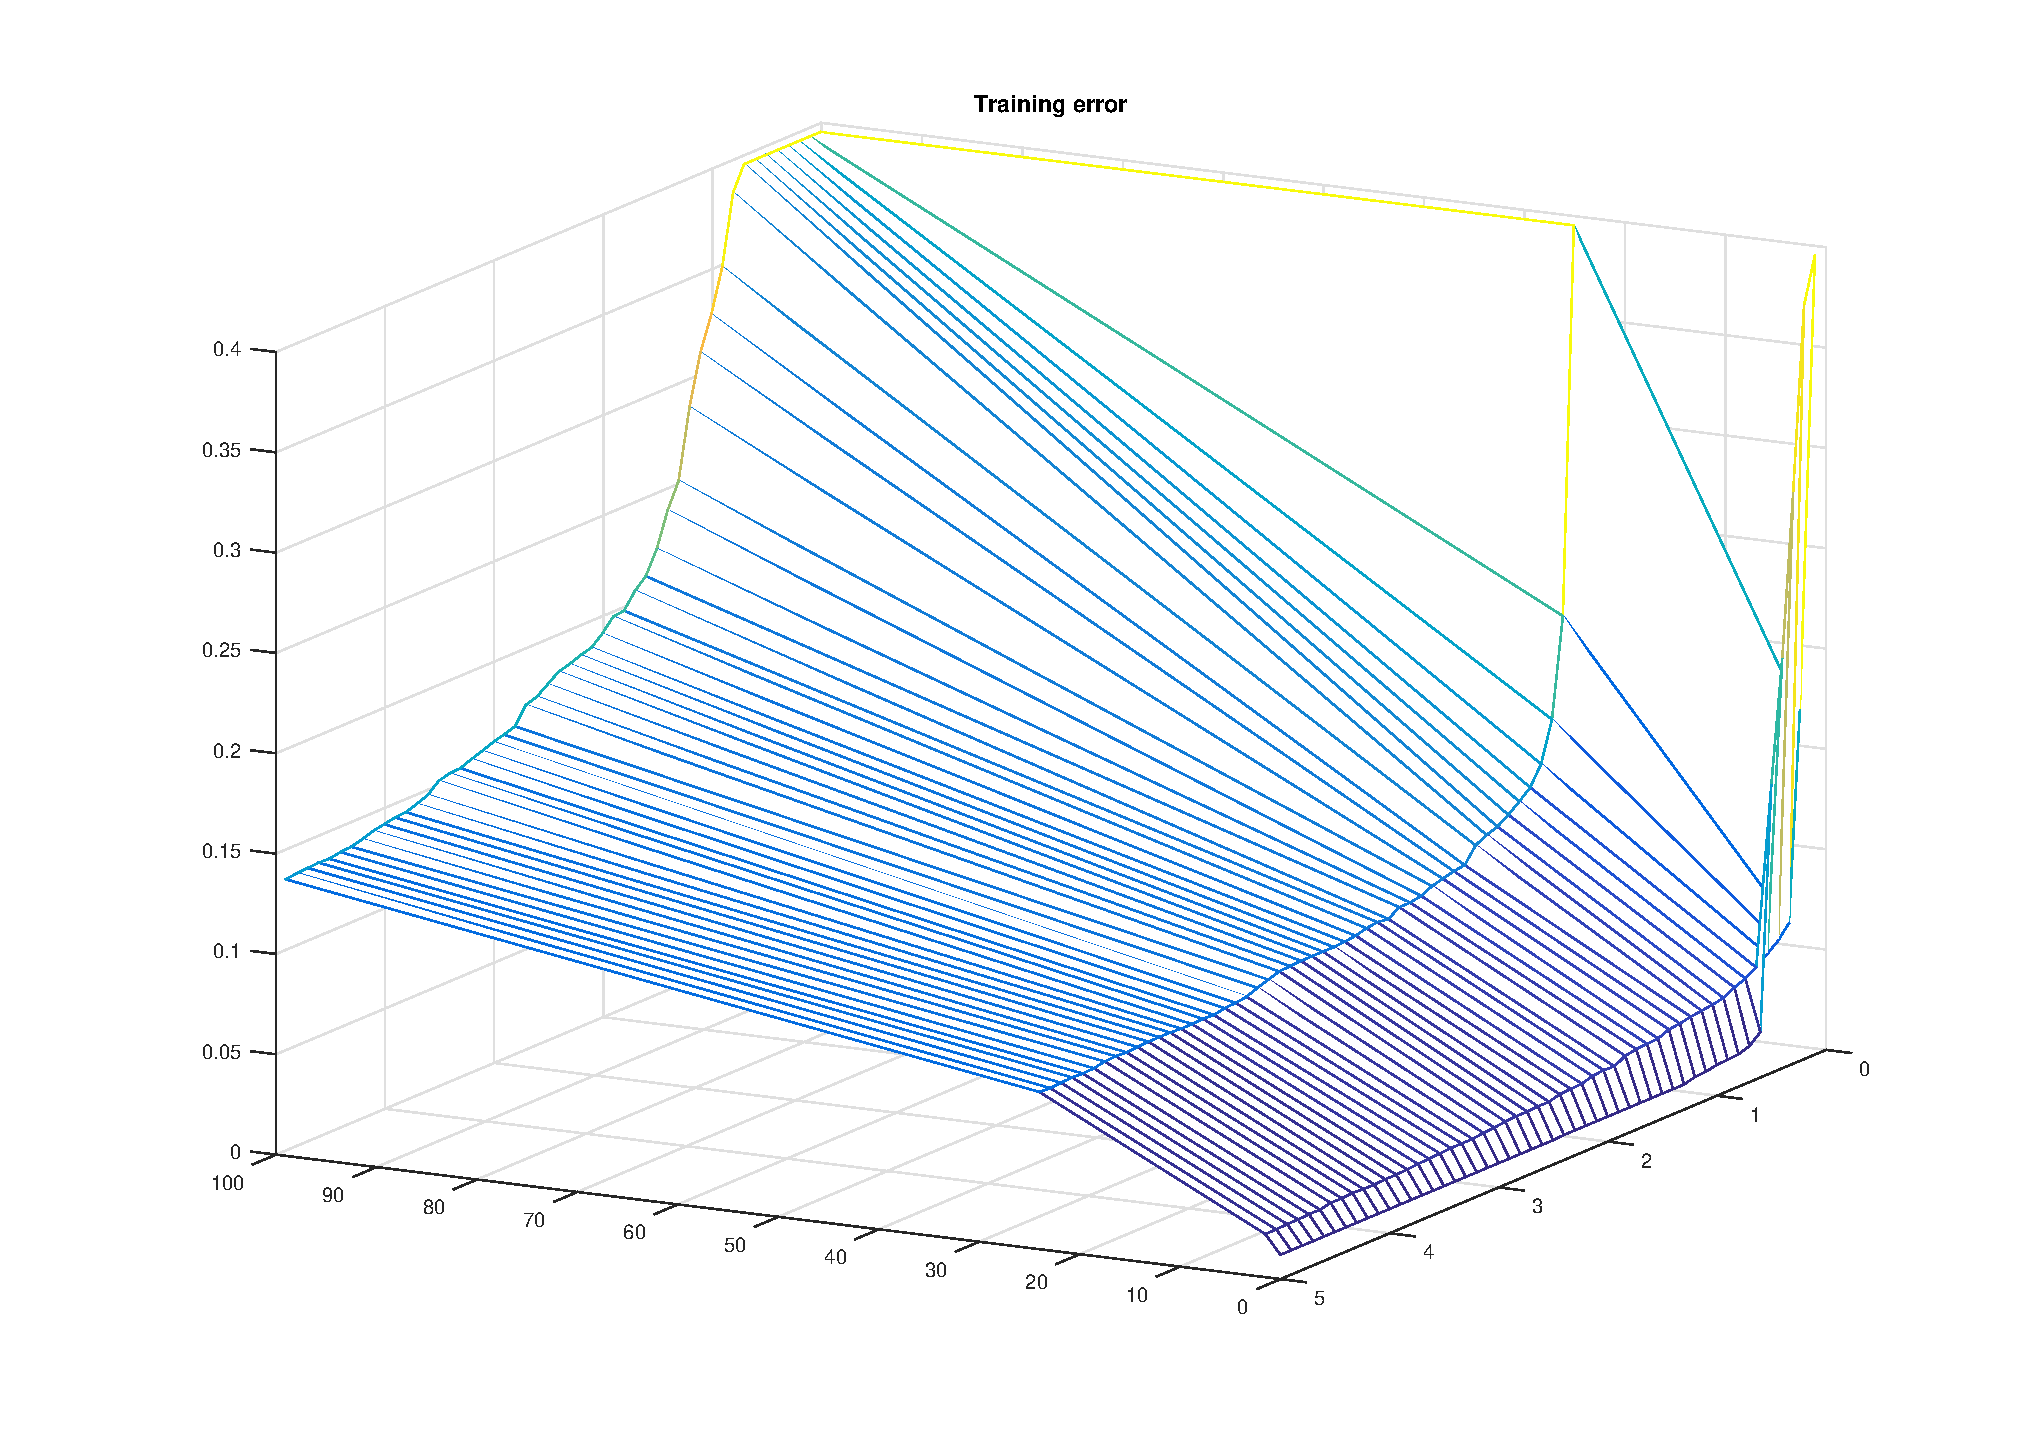
\includegraphics[width=0.47\textwidth]{../s1_svm/3_train_error.eps}
	\caption[]{\small Representación del error de clasificación respecto de $h$ y $P$}
	\label{fig:svm:p_h_optimo}
\end{figure}

Los valores óptimos son: $P=1.21$ y $h=2.5$.

El código generado es el siguiente:

\lstinputlisting{s1_ex3_report.m}

Una vez encontrado el clasificador óptimo, sobre la base de datos de test, el error obtenido es de $p_{e_{test}} = 0.0543478$. En comparación con la probabilidad encontrada en la primera ejecución ($p_e = 0.34891$), el clasificador óptimo mejora sustancialmente el rendimiento de la clasificación.

\section{Análisis de la bondad del clasificador}

Los indicadores de clasificación obtenidos con los parámetros óptimos son:

\begin{align}
	Ec &= 0.0543 \\
	A &= 0.9457 \\
	P &= 0.9377 \\
	S &= 0.9348 \\
	Es &= 0.9608 \\
	Fscore &= 0.9298
\end{align}

Para un caso en que se tengan 400 vectores SPAM y 4600 vectores MAIL, usar los cocientes $P$, $S$, $E_s$ y $F_{score}$ es más adecuado porque los errores al clasificar SPAM como MAIL serán escasos, ya que hay pocos ejemplos de SPAM, respecto de MAIL.

Esto hará que este tipo de errores tenga poca relevancia respecto la clasificación de los ejemplos de MAIL.

Los cocientes $P$, $S$, $E_s$ y $F_{score}$ valoran el comportamiento de la clasificación, fijándose en una clase cada vez, de manera que la proporción entre los ejemplos de una clase y otra no se tienen en cuenta.

\section{Análisis de la validez de decisión}

Las probabilidades a priori de las dos clases, después de clasificar son:

\begin{align}
	P_{mail} &= 0.5848 \\
	P_{spam} &= 0.4152
\end{align}


La predicción del vector de análisis ha sido $V_{analisis_{pred}} = 0 (MAIL)$. El parámetro $Pred_{validity} = 1$ indica que la predicción es correcta.

El vector no contiene la palabra "Make" ni la palabra "Address".

\newpage

La probabilidad a posteriori es de:

\begin{equation}
	\begin{aligned}
		P\left(A | B\right) &\equiv Pr \left\lbrace V_{analisis}=MAIL | clasificador=MAIL \right\rbrace \\
		P\left(A | B\right) &= \frac{P \left( B | A \right) \cdot P \left( A \right)}{P \left( B \right)} \\
		P \left( B | A \right) & \equiv Pr \left\lbrace clasificador=MAIL | V_{analisis}=MAIL \right\rbrace \equiv S\\
		P \left( A \right) &= \frac{N_{mail}}{N_{train}}, or \frac{N_{spam}}{N_{train}} \\
		P \left( B \right) &= P_{mail} , or P_{spam}
	\end{aligned}
\end{equation}

Para el caso de $V_{analisis}$, los valores de las probabilidades son:

\begin{align}
	P \left( A \right) &= 0.6014 \\
	P \left( B \right) &= 0.5848 \\
	P \left( B | A \right) &= 0.9348 \\
	P\left(A | B\right) &= 0.9615
\end{align}

El código que genera estos datos es el siguiente:

\lstinputlisting{s3_ex3_report.m}

\end{document}
 